\documentclass[11pt]{article}
\usepackage[margin=1in]{geometry}
\usepackage{amsmath,amssymb}
\usepackage{tikz}
\usepackage{pgfplots}
\usepackage{booktabs}
\usepackage{xcolor}
\usepackage{float}

\usetikzlibrary{patterns,decorations.pathmorphing,calc,arrows.meta,shadows,positioning}

% Brand colors
\definecolor{garnet}{HTML}{73000A}
\definecolor{atlantic}{HTML}{466A9F}
\definecolor{congaree}{HTML}{1F414D}
\definecolor{horseshoe}{HTML}{65780B}
\definecolor{rose}{HTML}{CC2E40}
\definecolor{black90}{HTML}{363636}
\definecolor{black70}{HTML}{5C5C5C}
\definecolor{black50}{HTML}{A2A2A2}
\definecolor{black30}{HTML}{C7C7C7}
\definecolor{honeycomb}{HTML}{A49137}
\definecolor{sandstorm}{HTML}{FFF2E3}
\definecolor{grass}{HTML}{CED318}

\pgfplotsset{compat=1.18}

\newcommand{\degC}{$^\circ$C}
\newcommand{\unit}[1]{\,\mathrm{#1}}

\title{\textbf{Complete Heat Transfer Analysis:\\Cylinder in Square Enclosure with All Radiation Paths}}
\author{J.C. Vaught}
\date{\today}

\begin{document}
\maketitle

\section{Problem Statement}

Analyze heat loss from a steel cylinder enclosed in a plywood box, including \textbf{all} convective and radiative heat transfer paths:

\begin{table}[H]
\centering
\begin{tabular}{lll}
\toprule
\textbf{Parameter} & \textbf{Symbol} & \textbf{Value} \\
\midrule
Cylinder diameter & $D$ & $0.25\unit{m}$ \\
Cylinder temperature & $T_{cyl}$ & 90\degC{} (363 K) \\
Minimum air gap & $\delta$ & $0.10\unit{m}$ \\
Inner box side & $w_{in}$ & $0.45\unit{m}$ \\
Plywood thickness & $t$ & $0.01\unit{m}$ \\
Outer box side & $w_{out}$ & $0.47\unit{m}$ \\
Ambient temperature & $T_\infty$ & 20\degC{} (293 K) \\
Analysis length & $L$ & $0.30\unit{m}$ \\
\midrule
Steel emissivity (oxidized) & $\varepsilon_1$ & 0.80 \\
Plywood emissivity & $\varepsilon_2$ & 0.90 \\
\bottomrule
\end{tabular}
\end{table}

\section{Complete Thermal Network}

The complete thermal network includes \textbf{five} resistances with two parallel radiation paths:

\begin{figure}[H]
\centering
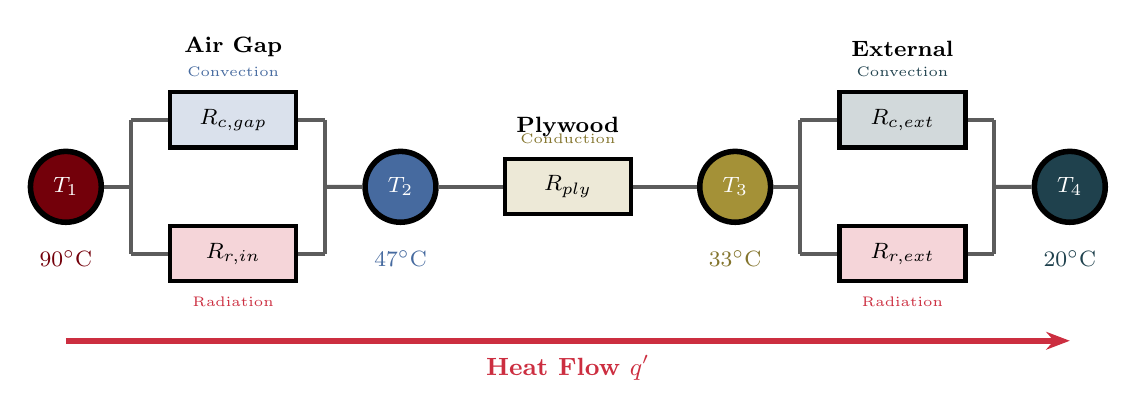
\begin{tikzpicture}[scale=0.85,
    node distance=1.8cm,
    res/.style={rectangle, draw, line width=1.5pt, minimum width=1.6cm, minimum height=0.7cm, font=\bfseries\footnotesize},
    temp/.style={circle, draw, line width=2pt, minimum size=0.9cm, font=\bfseries\footnotesize}
]
    % Temperature nodes
    \node[temp, fill=garnet, text=white] (T1) at (0,0) {$T_1$};
    \node[temp, fill=atlantic, text=white] (T2) at (5,0) {$T_2$};
    \node[temp, fill=honeycomb, text=white] (T3) at (10,0) {$T_3$};
    \node[temp, fill=congaree, text=white] (T4) at (15,0) {$T_4$};

    % Labels below
    \node[below=0.2cm of T1, garnet, font=\footnotesize] {90\degC};
    \node[below=0.2cm of T2, atlantic, font=\footnotesize] {47\degC};
    \node[below=0.2cm of T3, honeycomb!80!black, font=\footnotesize] {33\degC};
    \node[below=0.2cm of T4, congaree, font=\footnotesize] {20\degC};

    % === AIR GAP SECTION ===
    \draw[line width=1.5pt, black70] (T1.east) -- ++(0.4,0) coordinate (split1);
    \draw[line width=1.5pt, black70] (split1) -- ++(0,1) coordinate (top1);
    \draw[line width=1.5pt, black70] (split1) -- ++(0,-1) coordinate (bot1);

    % Convection resistance (air gap)
    \node[res, fill=atlantic!20] (Rconv1) at (2.5,1) {$R_{c,gap}$};
    \draw[line width=1.5pt, black70] (top1) -- (Rconv1.west);

    % Radiation resistance (inner)
    \node[res, fill=rose!20] (Rrad1) at (2.5,-1) {$R_{r,in}$};
    \draw[line width=1.5pt, black70] (bot1) -- (Rrad1.west);

    % Rejoin
    \draw[line width=1.5pt, black70] (Rconv1.east) -- ++(0.4,0) coordinate (top2);
    \draw[line width=1.5pt, black70] (Rrad1.east) -- ++(0.4,0) coordinate (bot2);
    \draw[line width=1.5pt, black70] (top2) -- ++(0,-1) coordinate (join1);
    \draw[line width=1.5pt, black70] (bot2) -- ++(0,1);
    \draw[line width=1.5pt, black70] (join1) -- (T2.west);

    % === PLYWOOD SECTION ===
    \node[res, fill=honeycomb!20] (Rply) at (7.5,0) {$R_{ply}$};
    \draw[line width=1.5pt, black70] (T2.east) -- (Rply.west);
    \draw[line width=1.5pt, black70] (Rply.east) -- (T3.west);

    % === EXTERNAL SECTION ===
    \draw[line width=1.5pt, black70] (T3.east) -- ++(0.4,0) coordinate (split2);
    \draw[line width=1.5pt, black70] (split2) -- ++(0,1) coordinate (top3);
    \draw[line width=1.5pt, black70] (split2) -- ++(0,-1) coordinate (bot3);

    % External convection
    \node[res, fill=congaree!20] (Rconv2) at (12.5,1) {$R_{c,ext}$};
    \draw[line width=1.5pt, black70] (top3) -- (Rconv2.west);

    % External radiation
    \node[res, fill=rose!20] (Rrad2) at (12.5,-1) {$R_{r,ext}$};
    \draw[line width=1.5pt, black70] (bot3) -- (Rrad2.west);

    % Rejoin to ambient
    \draw[line width=1.5pt, black70] (Rconv2.east) -- ++(0.4,0) coordinate (top4);
    \draw[line width=1.5pt, black70] (Rrad2.east) -- ++(0.4,0) coordinate (bot4);
    \draw[line width=1.5pt, black70] (top4) -- ++(0,-1) coordinate (join2);
    \draw[line width=1.5pt, black70] (bot4) -- ++(0,1);
    \draw[line width=1.5pt, black70] (join2) -- (T4.west);

    % Labels
    \node[above=0.05cm of Rconv1, atlantic, font=\tiny] {Convection};
    \node[below=0.05cm of Rrad1, rose, font=\tiny] {Radiation};
    \node[above=0.05cm of Rply, honeycomb!80!black, font=\tiny] {Conduction};
    \node[above=0.05cm of Rconv2, congaree, font=\tiny] {Convection};
    \node[below=0.05cm of Rrad2, rose, font=\tiny] {Radiation};

    % Section labels
    \node[above, font=\bfseries\footnotesize] at (2.5, 1.8) {Air Gap};
    \node[above, font=\bfseries\footnotesize] at (7.5, 0.6) {Plywood};
    \node[above, font=\bfseries\footnotesize] at (12.5, 1.8) {External};

    % Heat flow arrow
    \draw[-{Stealth[length=3mm]}, line width=2pt, rose] (0,-2.3) -- (15,-2.3);
    \node[rose, font=\bfseries\small] at (7.5,-2.7) {Heat Flow $q'$};

\end{tikzpicture}
\caption{Complete thermal resistance network with parallel convection and radiation at both the air gap and external surfaces.}
\label{fig:network}
\end{figure}

\section{Surface Areas and View Factors}

Per unit length:
\begin{align}
    A_1 &= \pi D = \pi \times 0.25 = 0.785\unit{m^2/m} && \text{(cylinder)} \\
    A_2 &= 4 w_{in} = 4 \times 0.45 = 1.80\unit{m^2/m} && \text{(inner box)} \\
    A_3 &= 4 w_{out} = 4 \times 0.47 = 1.88\unit{m^2/m} && \text{(outer box)}
\end{align}

View factors:
\begin{itemize}
    \item $F_{1 \to 2} = 1$ (cylinder completely enclosed by inner box)
    \item $F_{3 \to surr} = 1$ (outer box is convex, radiates to large surroundings)
\end{itemize}

\section{Resistance Calculations}

\subsection{Air Gap Convection ($R_{c,gap}$)}

Shape factor for cylinder in square enclosure:
\begin{equation}
    S = \frac{2\pi}{\ln(1.08 \cdot w_{in}/D)} = \frac{2\pi}{\ln(1.944)} = 9.45\unit{m^{-1}}
\end{equation}

Rayleigh and Nusselt numbers (with $\Delta T = 43$\degC):
\begin{align}
    Ra &= \frac{g\beta\Delta T \delta^3}{\nu\alpha} = 2.7 \times 10^6 \\
    Nu &= 0.046 \cdot Ra^{1/3} = 6.4 \\
    k_{eff} &= k_{air} \cdot Nu = 0.0283 \times 6.4 = 0.181\unit{W/(m \cdot K)}
\end{align}

\begin{equation}
    R_{c,gap} = \frac{1}{S \cdot k_{eff}} = \frac{1}{9.45 \times 0.181} = \boxed{0.583\unit{(m \cdot K)/W}}
\end{equation}

\subsection{Inner Radiation ($R_{r,in}$): Cylinder $\to$ Inner Plywood}

For enclosed radiation between cylinder and square box:
\begin{equation}
    \frac{1}{R_{r,in}} = \frac{\sigma(T_1^4 - T_2^4)}{T_1 - T_2} \cdot \frac{1}{\displaystyle\frac{1-\varepsilon_1}{\varepsilon_1 A_1} + \frac{1}{A_1} + \frac{1-\varepsilon_2}{\varepsilon_2 A_2}}
\end{equation}

Denominator terms:
\begin{align}
    \frac{1-\varepsilon_1}{\varepsilon_1 A_1} &= \frac{0.20}{0.80 \times 0.785} = 0.318 \\
    \frac{1}{A_1} &= 1.273 \\
    \frac{1-\varepsilon_2}{\varepsilon_2 A_2} &= \frac{0.10}{0.90 \times 1.80} = 0.062
\end{align}

Linearized radiation coefficient: $h_{r,in} = 7.0\unit{W/(m^2 \cdot K)}$

\begin{equation}
    R_{r,in} = \frac{1}{h_{r,in} \cdot A_1} = \frac{1}{7.0 \times 0.785} = \boxed{0.182\unit{(m \cdot K)/W}}
\end{equation}

\subsection{Combined Air Gap Resistance}

\begin{equation}
    R_{gap} = \left(\frac{1}{R_{c,gap}} + \frac{1}{R_{r,in}}\right)^{-1} = \left(\frac{1}{0.583} + \frac{1}{0.182}\right)^{-1} = \boxed{0.139\unit{(m \cdot K)/W}}
\end{equation}

\subsection{Plywood Conduction ($R_{ply}$)}

\begin{equation}
    R_{ply} = \frac{t}{k_{ply} \cdot A_2} = \frac{0.01}{0.12 \times 1.80} = \boxed{0.046\unit{(m \cdot K)/W}}
\end{equation}

\subsection{External Convection ($R_{c,ext}$)}

\begin{equation}
    R_{c,ext} = \frac{1}{h_{conv} \cdot A_3} = \frac{1}{7.0 \times 1.88} = \boxed{0.076\unit{(m \cdot K)/W}}
\end{equation}

\subsection{External Radiation ($R_{r,ext}$): Outer Plywood $\to$ Surroundings}

For a convex surface radiating to large surroundings:
\begin{equation}
    q_{rad} = \varepsilon_2 \sigma A_3 (T_3^4 - T_\infty^4)
\end{equation}

Linearized coefficient (at $T_3 \approx 33$\degC):
\begin{equation}
    h_{r,ext} = \varepsilon_2 \sigma (T_3^2 + T_\infty^2)(T_3 + T_\infty) = 0.9 \times 5.67 \times 10^{-8} \times (306^2 + 293^2)(306 + 293) = \boxed{5.5\unit{W/(m^2 \cdot K)}}
\end{equation}

\begin{equation}
    R_{r,ext} = \frac{1}{h_{r,ext} \cdot A_3} = \frac{1}{5.5 \times 1.88} = \boxed{0.097\unit{(m \cdot K)/W}}
\end{equation}

\subsection{Combined External Resistance}

\begin{equation}
    R_{ext} = \left(\frac{1}{R_{c,ext}} + \frac{1}{R_{r,ext}}\right)^{-1} = \left(\frac{1}{0.076} + \frac{1}{0.097}\right)^{-1} = \boxed{0.043\unit{(m \cdot K)/W}}
\end{equation}

\subsection{Total Resistance}

\begin{equation}
    R_{total} = R_{gap} + R_{ply} + R_{ext} = 0.139 + 0.046 + 0.043 = \boxed{0.228\unit{(m \cdot K)/W}}
\end{equation}

\section{Heat Loss Results}

\begin{equation}
    q' = \frac{T_{cyl} - T_\infty}{R_{total}} = \frac{90 - 20}{0.228} = \boxed{307\unit{W/m}}
\end{equation}

\begin{equation}
    Q = q' \times L = 307 \times 0.30 = \boxed{92\unit{W}}
\end{equation}

\section{Temperature Distribution}

\begin{align}
    T_1 &= 90\text{\degC} && \text{(cylinder)} \\
    T_2 &= T_1 - q' R_{gap} = 90 - 307 \times 0.139 = \boxed{47\text{\degC}} && \text{(inner plywood)} \\
    T_3 &= T_2 - q' R_{ply} = 47 - 307 \times 0.046 = \boxed{33\text{\degC}} && \text{(outer plywood)} \\
    T_4 &= 20\text{\degC} && \text{(ambient)}
\end{align}

\section{Model Comparison}

\begin{table}[H]
\centering
\caption{Effect of including radiation at each location}
\begin{tabular}{lccc}
\toprule
\textbf{Model} & \textbf{$R_{total}$ [(m$\cdot$K)/W]} & \textbf{$Q$ (30 cm) [W]} & \textbf{vs Base} \\
\midrule
1. Convection only & 0.705 & 29.8 & (base) \\
2. + Inner radiation & 0.261 & 80.5 & +170\% \\
3. + External radiation \textbf{(Complete)} & 0.228 & 92.3 & \textbf{+210\%} \\
\bottomrule
\end{tabular}
\end{table}

\begin{figure}[H]
\centering
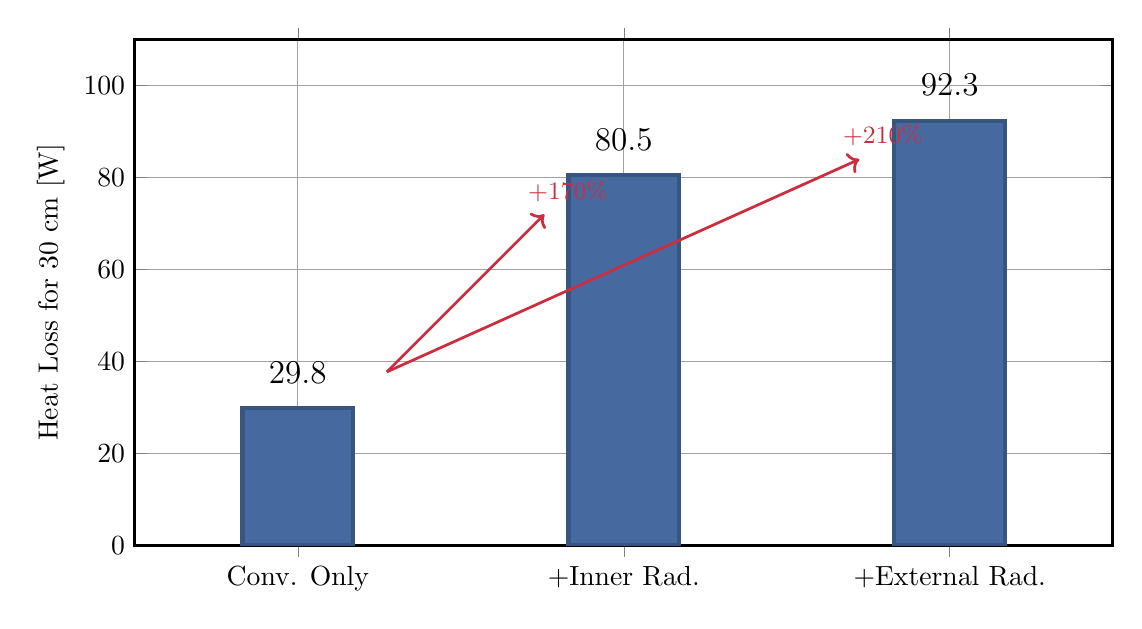
\begin{tikzpicture}
\begin{axis}[
    ybar,
    width=14cm,
    height=8cm,
    ylabel={Heat Loss for 30 cm [W]},
    symbolic x coords={Conv. Only, +Inner Rad., +External Rad.},
    xtick=data,
    ymin=0, ymax=110,
    bar width=40pt,
    nodes near coords,
    nodes near coords style={font=\bfseries\large},
    every node near coord/.append style={yshift=5pt},
    grid=both,
    grid style={line width=0.2pt, draw=black30},
    major grid style={line width=0.4pt, draw=black50},
    axis line style={line width=1pt},
    enlarge x limits=0.25,
    legend pos=north west,
]

\addplot[fill=atlantic, draw=atlantic!80!black, line width=1.5pt] coordinates {
    (Conv. Only, 29.8)
    (+Inner Rad., 80.5)
    (+External Rad., 92.3)
};

\end{axis}

% Annotations
\node[font=\small, rose] at (5.5, 4.5) {+170\%};
\node[font=\small, rose] at (9.5, 5.2) {+210\%};
\draw[->, line width=1pt, rose] (3.2, 2.2) -- (5.2, 4.2);
\draw[->, line width=1pt, rose] (3.2, 2.2) -- (9.2, 4.9);

\end{tikzpicture}
\caption{Heat loss increases significantly with each radiation path added.}
\end{figure}

\section{Resistance Breakdown}

\begin{table}[H]
\centering
\caption{Thermal resistance breakdown for complete model}
\begin{tabular}{lcccc}
\toprule
\textbf{Component} & \textbf{Resistance} & \textbf{Fraction} & \textbf{$\Delta T$} & \textbf{Effect of Radiation} \\
 & [(m$\cdot$K)/W] & & [\degC] & \\
\midrule
\multicolumn{5}{l}{\textit{Air Gap}} \\
\quad Convection only & 0.583 & -- & -- & -- \\
\quad Radiation only & 0.182 & -- & -- & -- \\
\quad \textbf{Combined} & \textbf{0.139} & \textbf{61\%} & \textbf{43} & $-76\%$ \\
\midrule
Plywood (conduction) & 0.046 & 20\% & 14 & -- \\
\midrule
\multicolumn{5}{l}{\textit{External}} \\
\quad Convection only & 0.076 & -- & -- & -- \\
\quad Radiation only & 0.097 & -- & -- & -- \\
\quad \textbf{Combined} & \textbf{0.043} & \textbf{19\%} & \textbf{13} & $-44\%$ \\
\midrule
\textbf{TOTAL} & \textbf{0.228} & \textbf{100\%} & \textbf{70} & \\
\bottomrule
\end{tabular}
\end{table}

\begin{figure}[H]
\centering
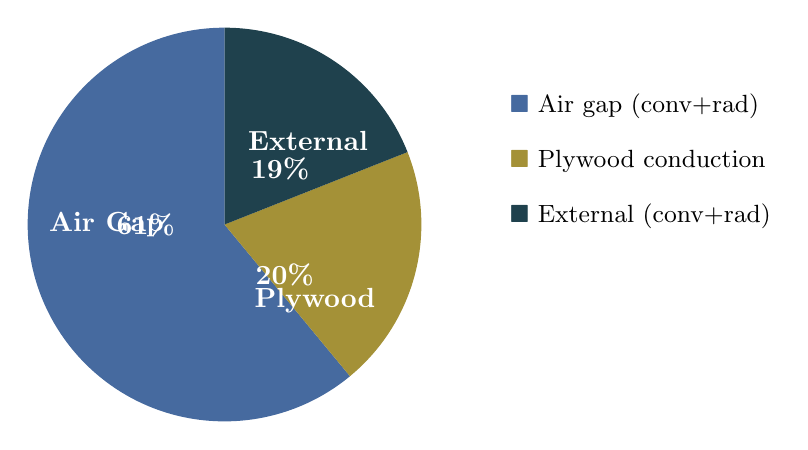
\begin{tikzpicture}
    % Pie chart
    \def\gapfrac{61}
    \def\plyfrac{20}
    \def\extfrac{19}

    \fill[atlantic] (0,0) -- (90:2.5) arc (90:90+0.61*360:2.5) -- cycle;
    \fill[honeycomb] (0,0) -- (90+0.61*360:2.5) arc (90+0.61*360:90+0.81*360:2.5) -- cycle;
    \fill[congaree] (0,0) -- (90+0.81*360:2.5) arc (90+0.81*360:90+360:2.5) -- cycle;

    \node[white, font=\bfseries] at (180:1.5) {Air Gap};
    \node[white, font=\bfseries] at (180:1.0) {61\%};

    \node[white, font=\bfseries] at (320:1.5) {Plywood};
    \node[white, font=\bfseries] at (320:1.0) {20\%};

    \node[white, font=\bfseries] at (45:1.5) {External};
    \node[white, font=\bfseries] at (45:1.0) {19\%};

    % Legend
    \node[right, font=\small] at (3.5,1.5) {\textcolor{atlantic}{$\blacksquare$} Air gap (conv+rad)};
    \node[right, font=\small] at (3.5,0.8) {\textcolor{honeycomb}{$\blacksquare$} Plywood conduction};
    \node[right, font=\small] at (3.5,0.1) {\textcolor{congaree}{$\blacksquare$} External (conv+rad)};

\end{tikzpicture}
\caption{Resistance distribution in the complete model.}
\end{figure}

\section{Key Findings}

\begin{enumerate}
    \item \textbf{Both radiation paths significantly increase heat loss}:
    \begin{itemize}
        \item Inner radiation (cylinder $\to$ inner plywood): +170\%
        \item External radiation (outer plywood $\to$ surroundings): additional +15\%
        \item \textbf{Total increase: +210\%} (from 30 W to 92 W)
    \end{itemize}

    \item \textbf{Inner radiation is dominant}: Reduces air gap resistance by 76\% (from 0.58 to 0.14).

    \item \textbf{External radiation is also significant}: Reduces external resistance by 44\% (from 0.076 to 0.043). The external radiation coefficient $h_{r,ext} = 5.5\unit{W/(m^2 \cdot K)}$ is comparable to convection $h_{conv} = 7\unit{W/(m^2 \cdot K)}$.

    \item \textbf{Final temperature profile}: 90\degC $\to$ 47\degC $\to$ 33\degC $\to$ 20\degC

    \item \textbf{Plywood provides 20\% of total resistance}: The main insulation comes from the air gap (61\%), even with radiation present.
\end{enumerate}

\section{Conclusions}

\begin{table}[H]
\centering
\caption{Final summary of heat loss for 30 cm cylinder length}
\begin{tabular}{lc}
\toprule
\textbf{Heat Transfer Model} & \textbf{Heat Loss [W]} \\
\midrule
Convection only (incomplete) & 30 \\
With inner radiation only (incomplete) & 81 \\
\textbf{Complete model (all paths)} & \textbf{92} \\
\bottomrule
\end{tabular}
\end{table}

The complete analysis shows that \textbf{radiation accounts for 68\% of total heat loss} (62 W out of 92 W). Ignoring either radiation path leads to significant underestimation:
\begin{itemize}
    \item Ignoring all radiation: underestimates by 68\%
    \item Ignoring external radiation only: underestimates by 13\%
\end{itemize}

\textbf{For design purposes}: To reduce heat loss, focus on reducing radiation, especially at the inner surface (low-emissivity coating on the cylinder or reflective barrier).

\end{document}
